\documentclass{article}
\usepackage[T1]{fontenc}
\usepackage{lmodern}
\usepackage{graphicx}
\usepackage{amsmath,amssymb}
\usepackage[a4paper,margin=2cm]{geometry}
\usepackage[absolute,overlay]{textpos}
\setlength{\TPHorizModule}{1mm}
\setlength{\TPVertModule}{1mm}
\usepackage[indonesian]{babel}
\usepackage{hyperref}
\setlength{\emergencystretch}{2em}
% unit: Halaman 43

\begin{document}

% === Halaman 43 (llm) ===

\vspace{136.62mm}

(a) Encryption
\vspace{80mm}
(b) Decryption

% deskripsi: Diagram blok proses enkripsi yang menunjukkan penggunaan shift register, blok enkripsi dengan kunci K, seleksi bit, dan operasi XOR dengan plaintext P untuk menghasilkan ciphertext C.
% bbox normalisasi: [0.1000, 0.0000, 0.9000, 0.4600]
\begin{textblock*}{168.00mm}(21.00mm,0.00mm)
\noindent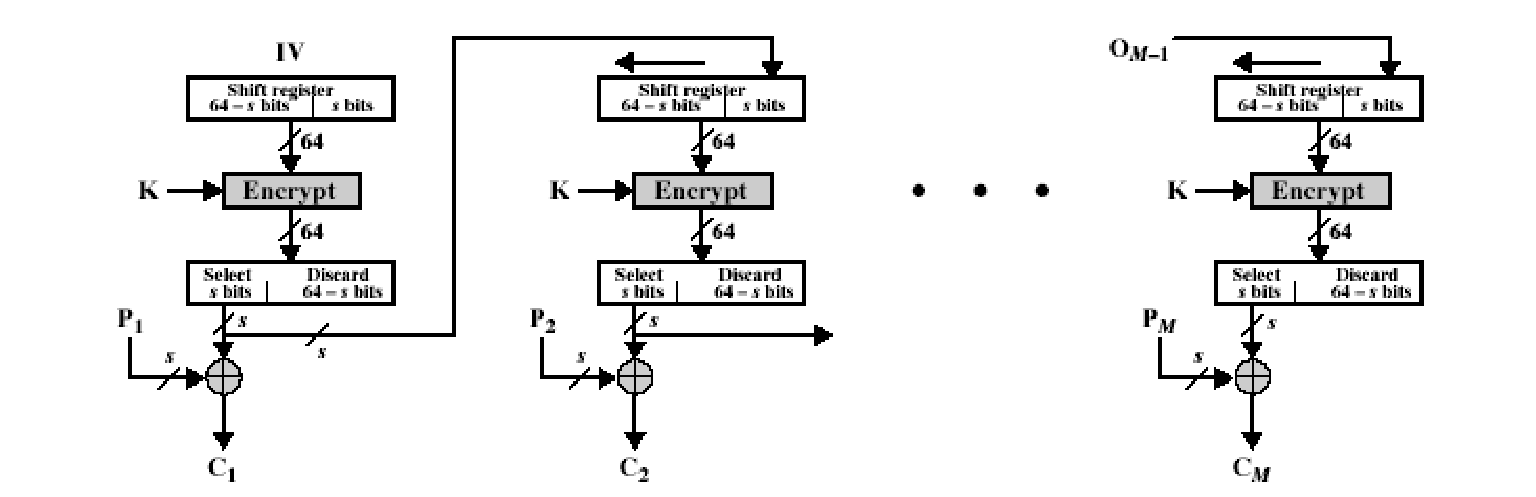
\includegraphics[width=168.00mm,height=136.62mm]{../../images/llm/page_043_img_01.png}%
\end{textblock*}

% deskripsi: Diagram blok proses dekripsi yang menunjukkan penggunaan shift register, blok dekripsi dengan kunci K, seleksi bit, dan operasi XOR dengan ciphertext C untuk mengembalikan plaintext P.
% bbox normalisasi: [0.1000, 0.5000, 0.9000, 0.9600]
\begin{textblock*}{168.00mm}(21.00mm,148.50mm)
\noindent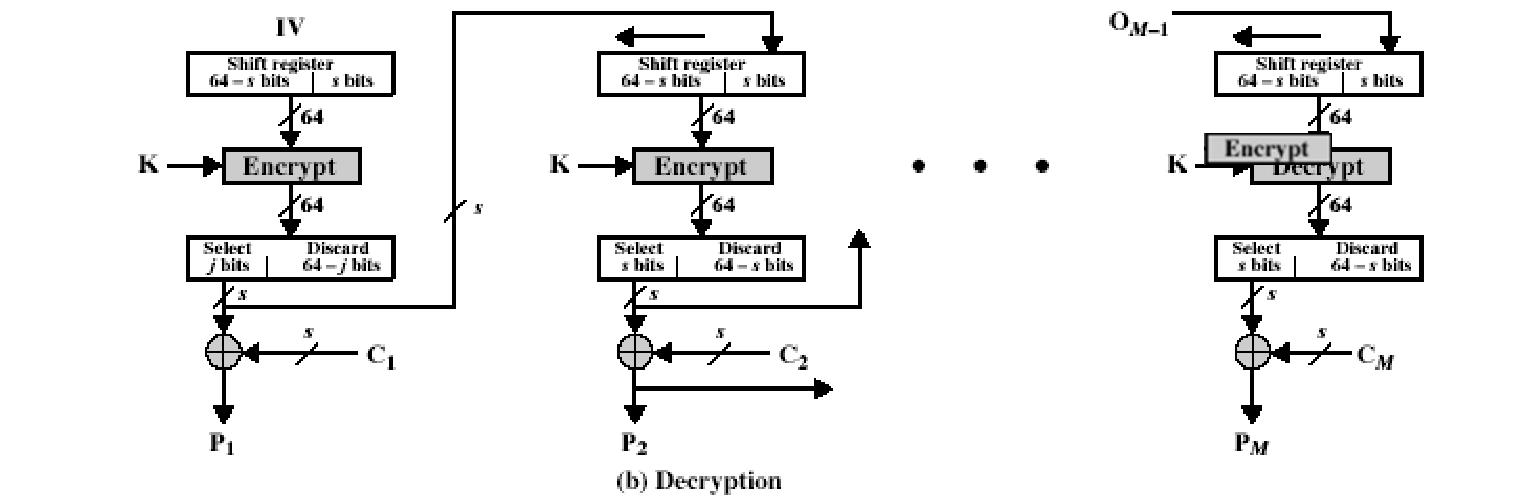
\includegraphics[width=168.00mm,height=136.62mm]{../../images/llm/page_043_img_02.png}%
\end{textblock*}

\end{document}
